\todo[inline,color=yellow]{Apresentar os resultados experimentais, inclua eventuais medidas de caracterização de componente (e.g., resistências, resistência parasítica do indutor). Avalie se é melhor apresentar o dado na forma de tabela ou gráfico. Note que um diagrama de Bode não deve ser apresentado na forma de tabela, enquanto que os valores de resistência utilizados poderiam utilizar este formato de apresentação.
}

\subsection{Nota}
	\todo[inline,color=yellow]{Caso apresente dados que serão usados para ajustar um modelo teórico, aproveite o espaço do gráfico para apresentar o ajuste. Faça uma breve discussão do ajuste,incluindo os parâmetros extraídos e equações utilizadas (evite deduções nesta parte). Sendo seu experimento constituído de mais de um conjunto de dados, utilize subseções.
}

\begin{figure}
	\centering
	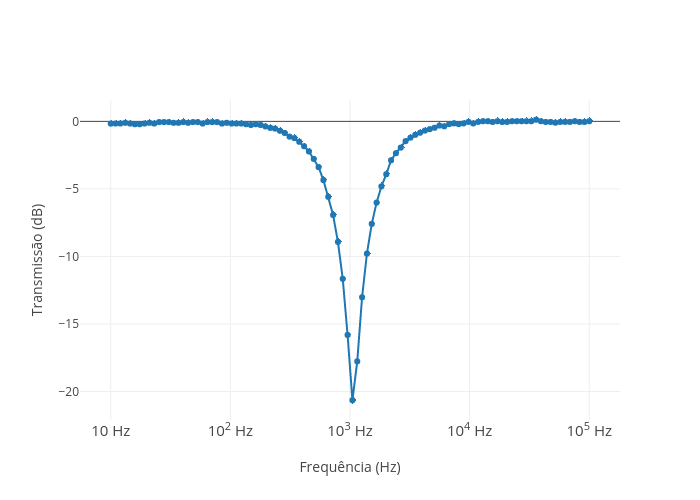
\includegraphics[width=0.9\textwidth]{figuras/diagrama-bode.png}
	\caption{
    	Diagrama de Bode
	}
    \label{fig:frog}
\end{figure}

\begin{center}
	\begin{tabular}{l|c}
    	\bfseries Frequência (Hz) & \bfseries Transmitância (dB)
     	\csvreader[head to column names]{dados/parte2.csv}{}
      	{\\\hline \freq & \TdB}
	\end{tabular}
\end{center}